\chapter{Sprint1}
\section{Introduction}
In this chapter, we will design and implement the functionalities of Sprint 1 of our project.
We will first present the sprint backlog, where we will detail the requested features. The next step is to analyze the specified functionalities. Finally, we will show the output of this sprint.
\section {Backlog Sprint}
\begin{table}[h]
\centering

\begin{tabular}{|c|p{5cm}|c|p{10cm}|}
\hline
ID & US & Estimation & Tâches à réaliser \\
\hline
 & & & \begin{tabular}[c]{@{}l@{}}
 - Setting up the work environment
    \\- Preparing the project structure Backend
    \\- Preparing the libraries and creating the REST APIs
    \\ - Preparing the database \end{tabular} \\
\hline
1 & as a collaborator, I want to authenticate to the platform & 3 &\begin{tabular}[c]{@{}l@{}}- Creation of the graphical interface (UX) for authentication for \\ an Orange collaborator Administrator/Coordinator/Exepert\\

-Implement the interface
\\-Implement the necessary methods to ensure user authentication
\\-Test \end{tabular}\\
\hline
2 & as a collaborator, I want to logout of the platform & 2 & \begin{tabular}[c]{@{}l@{}} Creation of the graphical interface (UX) for logout for \\an Orange collaborator Administrator/Coordinator/Exepert\\

    -Implement the interface
    \\-Implement the necessary methods to ensure user logout
    \\-Test \end{tabular}\\
\hline
3 & As a collaborator, I want to update my profile &2 & \begin{tabular}[c]{@{}l@{}}- Creation of the graphical interface (UX) for updating profile \\
    - Implement the interface \\
    - Implement the necessary methods to update profile details \\
    - Test \end{tabular} \\
\hline
4 & As an ODC collaborator, I want to change my password &1& \begin{tabular}[c]{@{}l@{}}- Creation of the graphical interface (UX) for changing password \\
    - Implement the interface \\
    - Implement the necessary methods to change password \\
    - Test \end{tabular} \\
    \hline     
\end{tabular}

\end{table}
\newpage 
\begin{table}[h]
    \centering
    \begin{tabular}{|c|p{5cm}|c|p{10cm}|}
        \hline
        ID & US & Estimation & Tâches à réaliser \\
        \hline
        5 & As a super admin, I want to add an ODC coordinator & 2& \begin{tabular}[c]{@{}l@{}}- Creation of the graphical interface (UX) for adding an ODC\\ coordinator \\
            - Implement the interface \\
            - Implement the necessary methods to add an ODC coordinator \\
            - Test \end{tabular} \\
            \hline
    6 &\begin{tabular}[c]{@{}l@{}} As a super admin,\\ I want to enable/disable \\an ODC collaborator \\coordinator/Expert \end{tabular} & 3& \begin{tabular}[c]{@{}l@{}}- Creation of the graphical interface (UX) for enabling/disabling an \\ODC collaborator coordinator/Expert \\
        - Implement the interface \\
        - Implement the necessary methods to enable/disable an ODC \\collaborator coordinator/Expert \\
        - Test \end{tabular} \\
        \hline
        7 &  As a super admin,I want to view ODC Coordinators/Experts list & 3& \begin{tabular}[c]{@{}l@{}}- Creation of the graphical interface (UX) for viewing \\ODC coordinator/experts list \\
            - Implement the interface \\
            - Implement the necessary methods to view ODC experts list \\
            - Test \end{tabular} \\
            \hline
        7 & As an ODC Coordinator, I want to add an ODC Expert &2& \begin{tabular}[c]{@{}l@{}}- Creation of the graphical interface (UX) for adding an\\ ODC Expert \\
            - Implement the interface \\
            - Implement the necessary methods to add an ODC Expert \\
            - Test \end{tabular} \\
            \hline        
            8 & As an ODC Coordinator, I want to enable/disable an ODC Expert &2 & \begin{tabular}[c]{@{}l@{}}- Creation of the graphical interface (UX) for enabling\\/disabling an ODC Expert \\
                - Implement the interface \\
                - Implement the necessary methods to enable/disable \\an ODC Expert \\
                - Test \end{tabular} \\
                \hline
                9 & As an ODC Coordinator,I want to view ODC experts list &2 & \begin{tabular}[c]{@{}l@{}}- Creation of the graphical interface (UX) for viewing \\ODC experts list \\
                    - Implement the interface \\
                    - Implement the necessary methods to view ODC experts list \\
                    - Test \end{tabular} \\
                    \hline
                
    \end{tabular}
    \caption{Backlog for the First Sprint}
\label{tab:Backlog for the First Sprint}
\end{table}
\newpage
\section{Use Case Diagram for Sprint 1} 
The following figure represents the use case diagram for our first sprint.
\begin{figure}[h!]
    \centering
    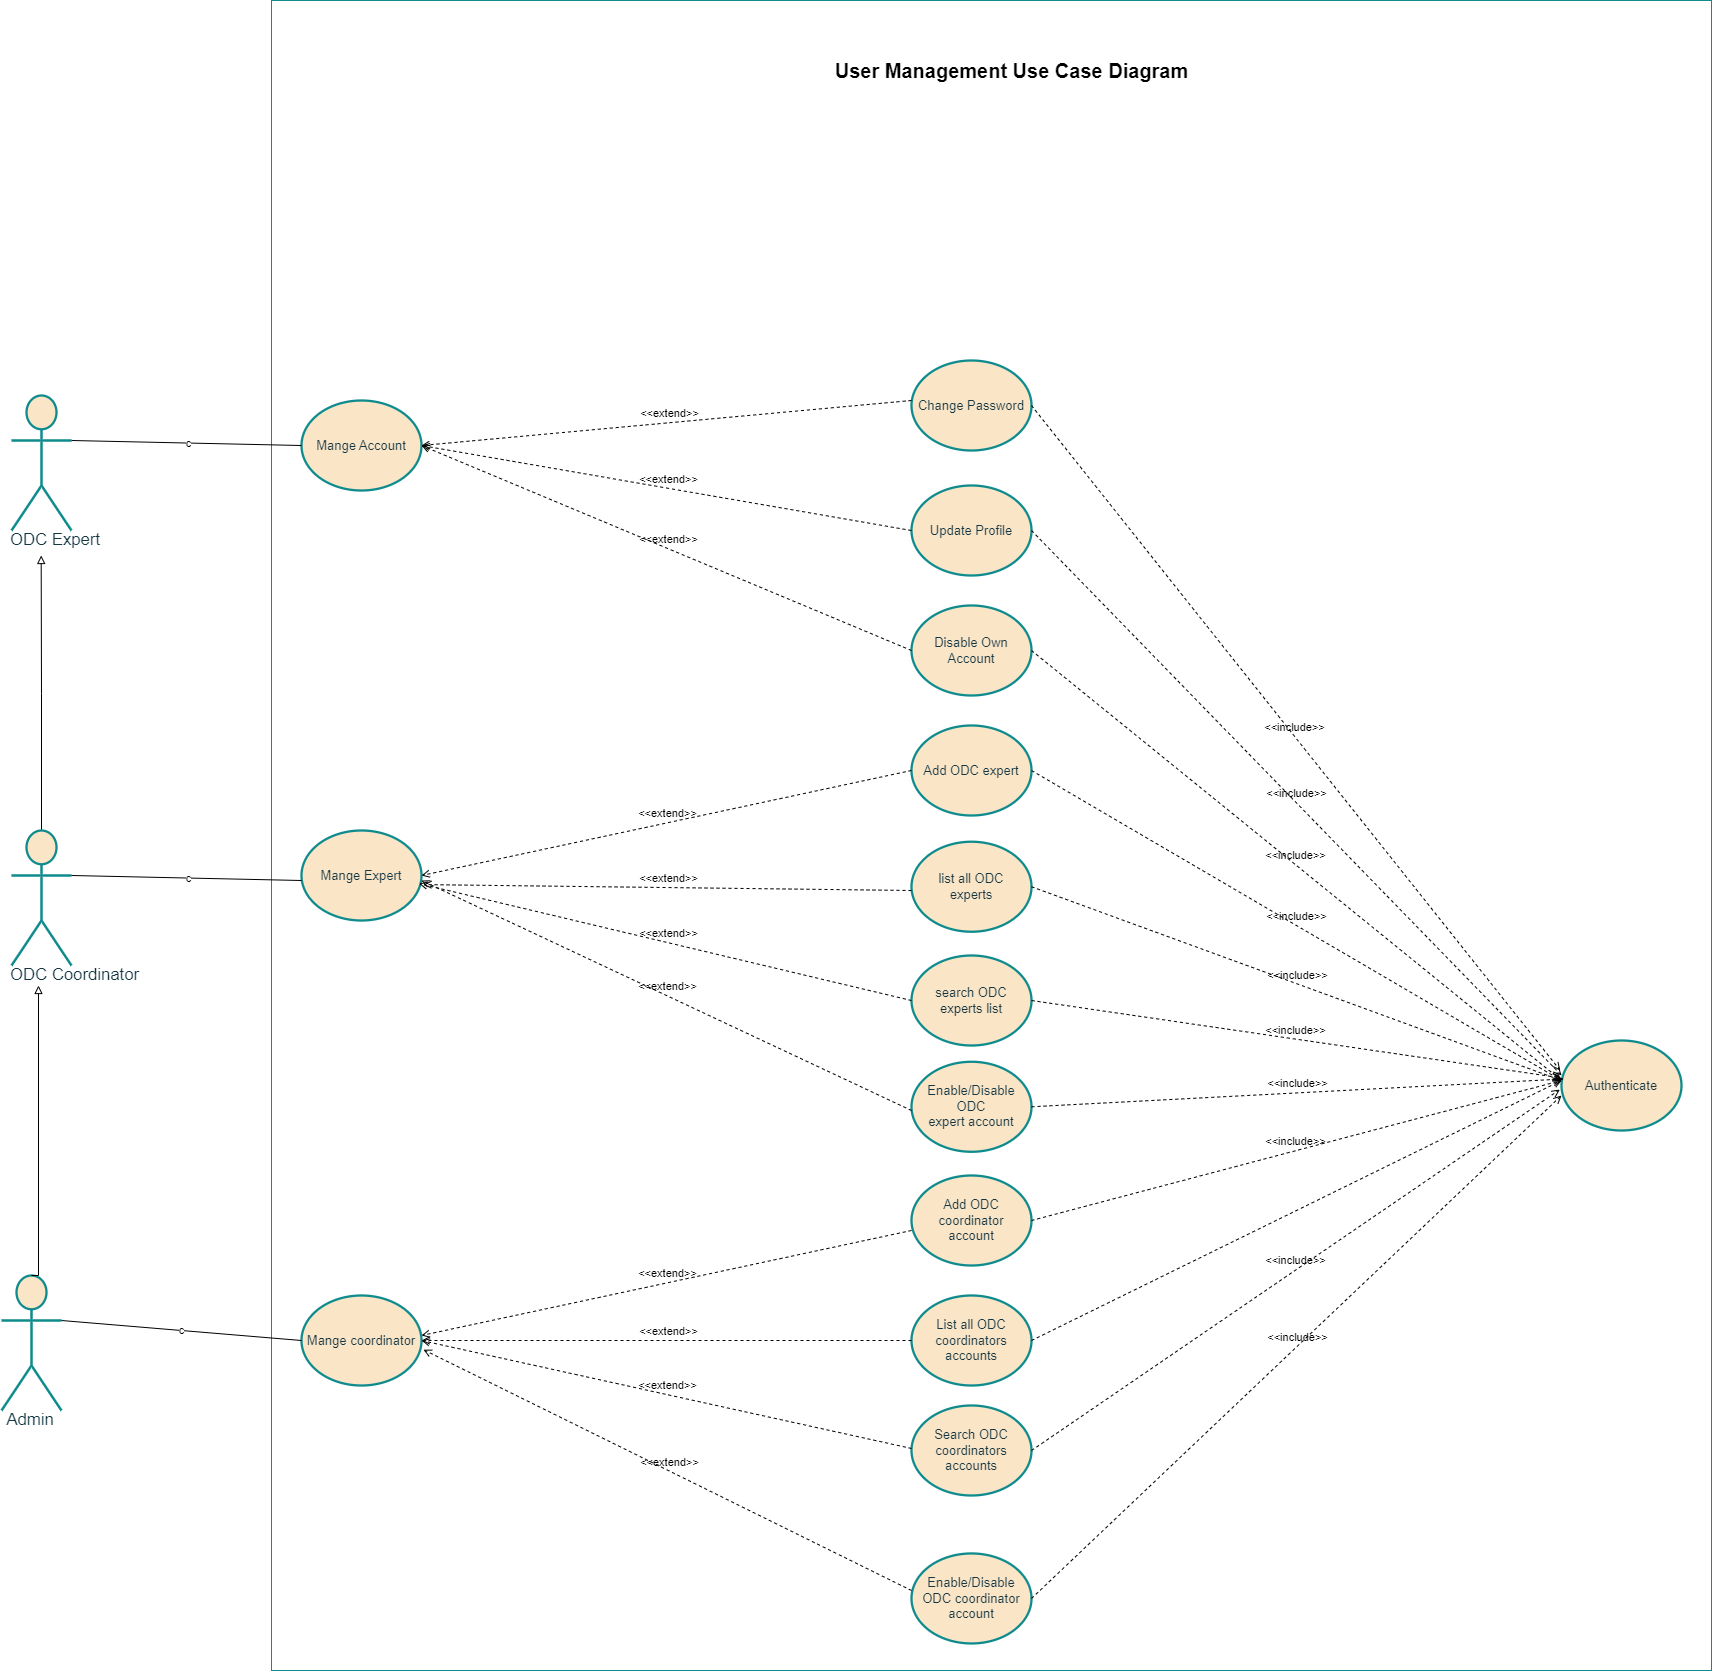
\includegraphics[height=1\textwidth]{images/usecaseS1.png}
    \caption{Use Case Diagram for Sprint 1}
    \label{fig:Use Case Diagram for Sprint 1}
\end{figure}
\newpage 

\subsection{Textual Description of the Use Case "Authenticate"}
\begin{table}[h]
    \centering
    \begin{tabular}{|c|c|}
        \hline
        Use Case & authenticate \\
        \hline
    Actor &\begin{tabular}[c]{@{}l@{}} User: Collaborator/Administrator


    \end{tabular} \\
        \hline
        Brief Description &\begin{tabular}[c]{@{}l@{}} The user must be registered in the database and must know their credentials
        \end{tabular} \\
            \hline
            Pre-condition &\begin{tabular}[c]{@{}l@{}} The user must have their access parameters
            \end{tabular} \\
                \hline
                Post-condition &\begin{tabular}[c]{@{}l@{}} The user is successfully authenticated
                \end{tabular} \\
                    \hline
                    Main Scenario &\begin{tabular}[c]{@{}l@{}} 1. The user enters their credentials (email and password) in the appropriate fields \\and submits the form.
                       \\ 2. The system verifies the information entered by the user
                        \\3. The system displays the appropriate interface according to the role of the user
                    \end{tabular} \\
                        \hline
                        Exception Scenario &\begin{tabular}[c]{@{}l@{}} 1.1 The entered data is incorrect or missing:
                          \\  2.1.1 The system displays an error message and the use case returns to step 1 of the main scenario
                            \\2.1 The entered credentials do not exist in the database:
                            \\2.1.1 The system displays an error message and the use case returns to step 2 of the main scenario
                        \end{tabular} \\
                            \hline
                            Extension &\begin{tabular}[c]{@{}l@{}} In case of forgotten password, the user can redefine a new password
                            \end{tabular} \\
                                \hline
                                
    \end{tabular}
    
    \begin{center}
        \caption{Textual Description of the Use Case "Authenticate"}
        \label{tab:Textual Description of the Use Case "Authenticate"}
        \end{center}    
    \end{table}
    \subsection{the sequence diagram for the use case 'authenticate'}
    
    \begin{figure}[h!]
        \centering
        "The following figure represents the sequence diagram for the use case 'authenticate'."\\
        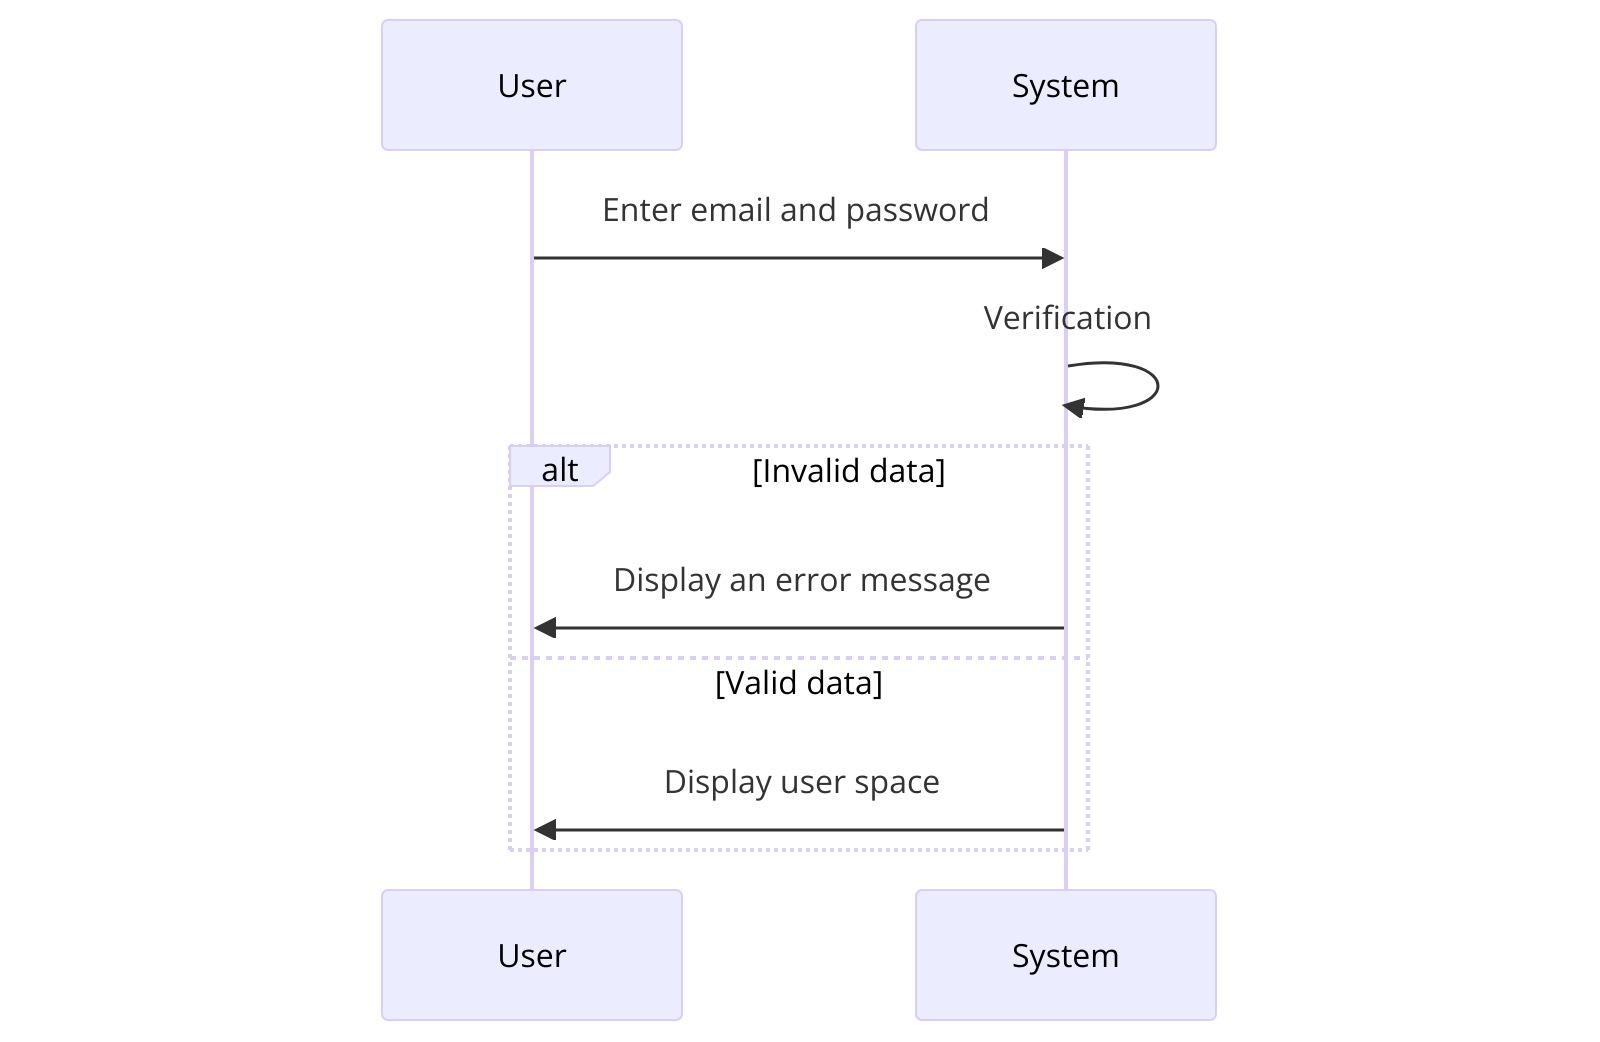
\includegraphics[width=0.8\textwidth]{images/diagram seq.png}
        \caption{the sequence diagram for the use case 'authenticate'}
        \label{fig:the sequence diagram for the use case 'authenticate'}
  \end{figure}






   
    \newpage
    Each user who wants to authenticate must access the authentication page. Then, they enter their email and password. The system validates and verifies their existence. If these credentials are valid, a message indicating that the user must activate their account via email is sent. The user then checks their email inbox and clicks on the received link to securely access their personal space. Otherwise, an error message is displayed indicating that the entered data is invalid.


    \subsection{Textual Description of the Use Case "Add Coordinator"}

    \begin{table}[h]
        \centering
        \begin{tabular}{|c|p{12cm}|}
            \hline
            Use Case & Add Coordinator \\
            \hline
            Actor & \begin{tabular}[c]{@{}l@{}} 
                Super Admin \\ 
                Coordinator     
            \end{tabular} \\
            \hline
            Brief Description & The Super Admin adds a new coordinator by providing the necessary details. The coordinator receives an email to set up their password. \\
            \hline
            Pre-condition & The Super Admin must be authenticated and have the necessary permissions. \\
            \hline
            Post-condition & The coordinator is successfully added and can log in after setting up their password. \\
            \hline
            Main Scenario & \begin{tabular}[c]{@{}l@{}} 
                1. The Super Admin accesses the "Add New Coordinator" page. \\
                2. The Super Admin fills in the fields: name, last name, country, email. \\
                3. The Super Admin presses the "Add" button. \\
                4. The system validates the entered information. \\
                5. The system sends an email to the new coordinator. \\
                6. The coordinator receives the email and clicks the link. \\
                7. The coordinator is redirected to the password setup page. \\
                8. The coordinator sets up the password. \\
                9. The coordinator is redirected to the login page.
            \end{tabular} \\
            \hline
            Exception Scenario & \begin{tabular}[c]{@{}l@{}} 
                2.1 The entered data is incorrect or missing: \\
                2.1.1 The system displays an error message and the use case returns to step 2\\ of the main scenario. \\
                4.1 The entered email is already in use or invalid: \\
                4.1.1 The system displays an error message and the use case returns to step 2\\ of the main scenario.
            \end{tabular} \\
            \hline
            Extension & In case of forgotten password, the coordinator can redefine a new password. \\
            \hline
        \end{tabular}
        \begin{center}
            \caption{Textual Description of the Use Case "Add Coordinator"}
            \label{tab:Textual Description of the Use Case "Add Coordinator"}
            \end{center}    
    \end{table}
  
    \newpage
\subsection{Sequence Diagram of the Use Case 'Add Coordinator'}

\begin{figure}[h!]
    \centering
    "The following figure represents the sequence diagram for the use case 'Add Coordinator'\\
    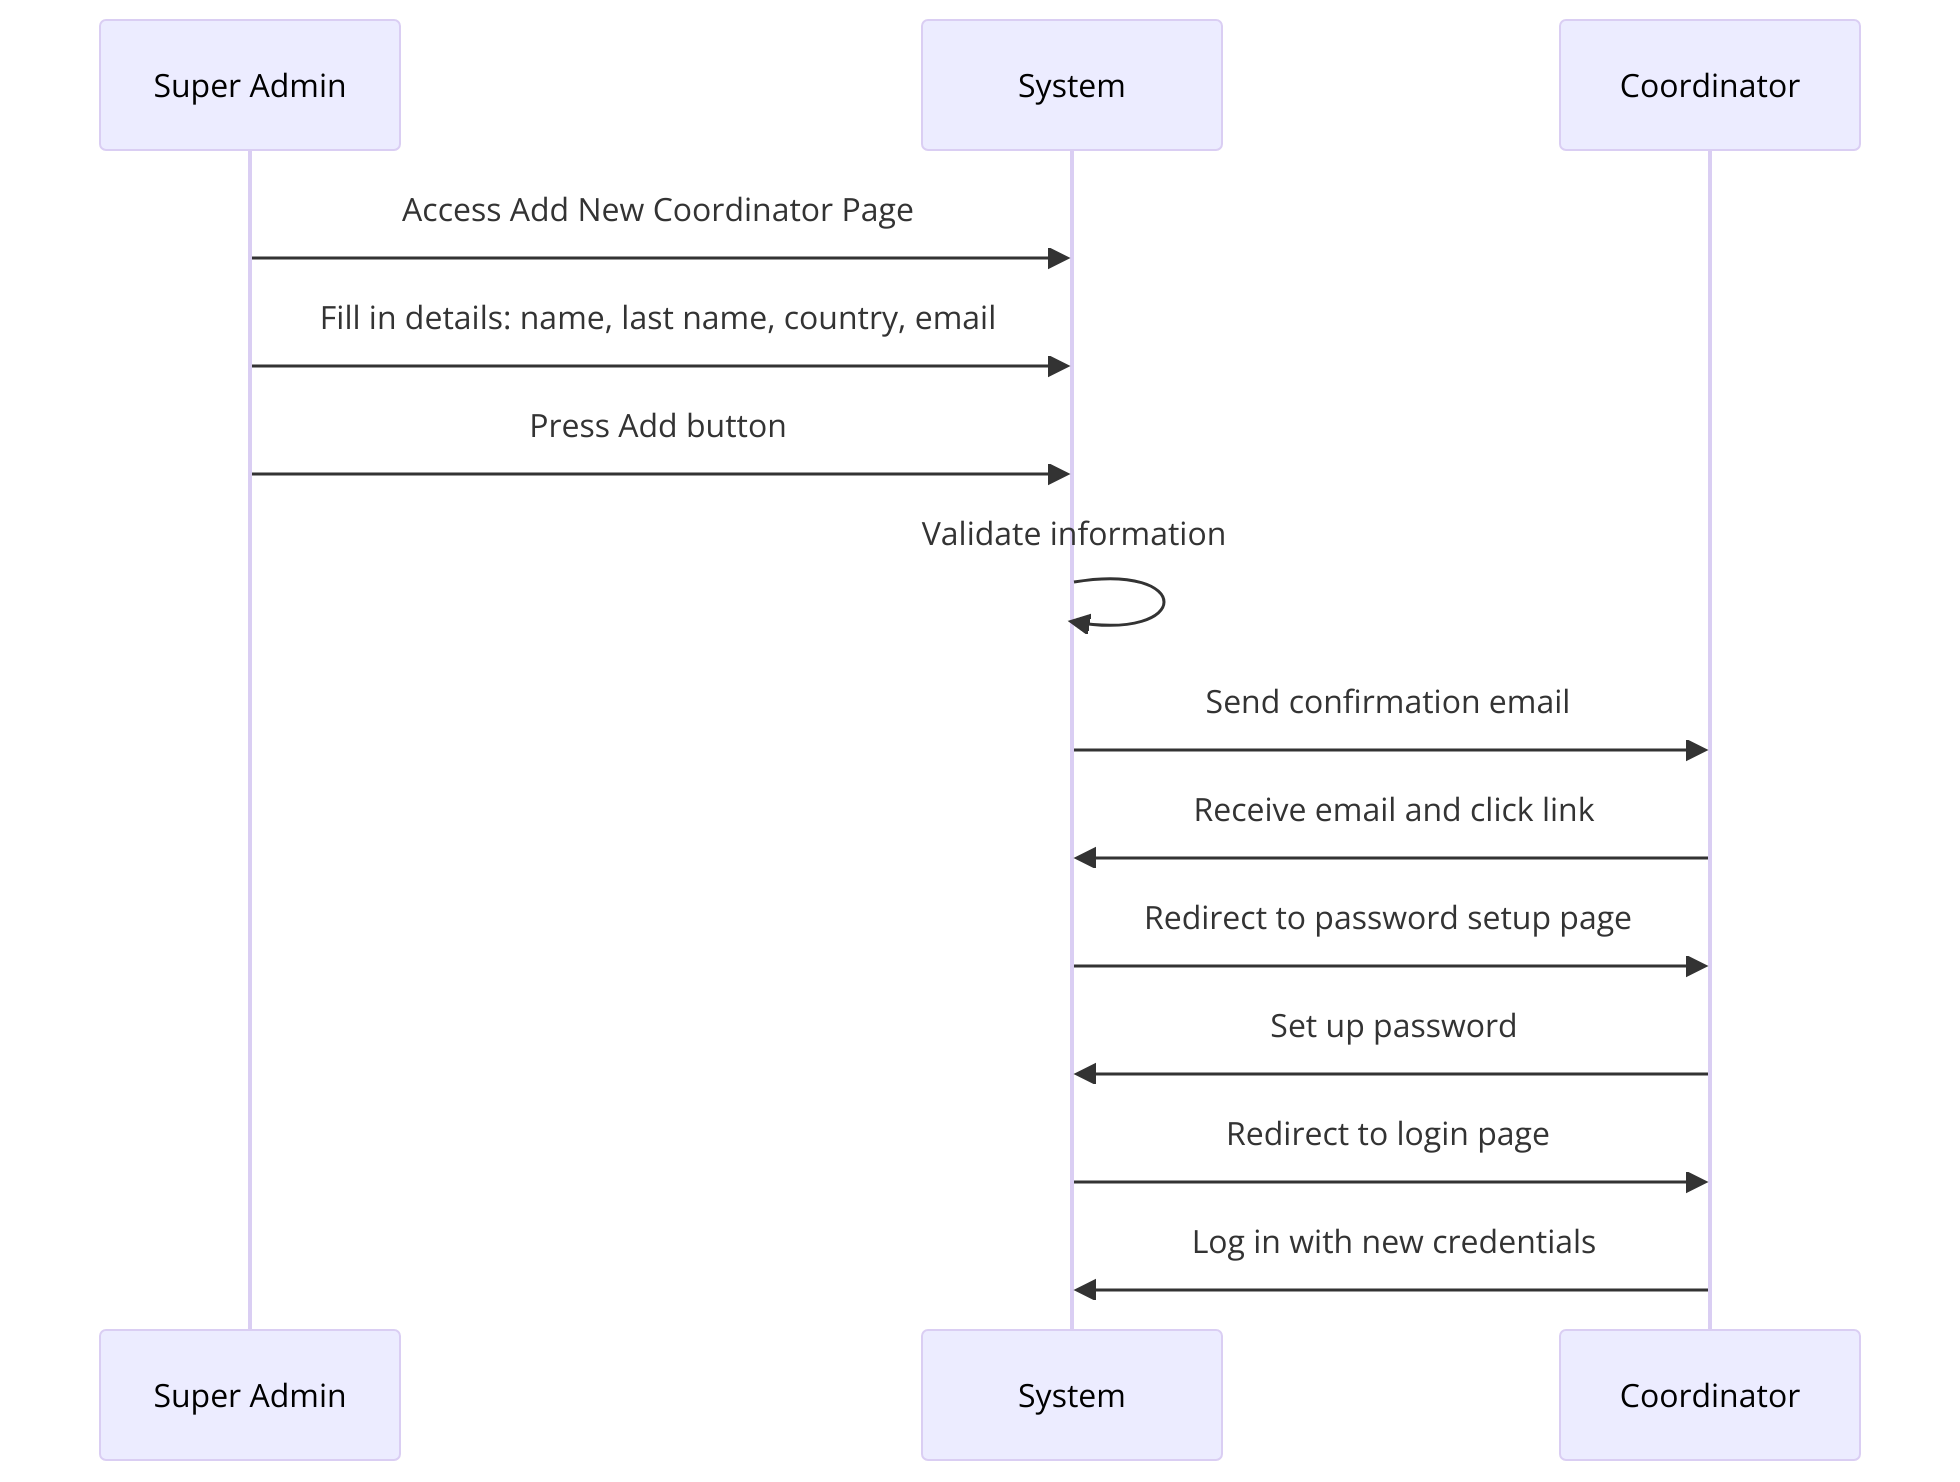
\includegraphics[width=0.8\textwidth]{images/diagram seq2.png}
    \caption{the sequence diagram for the use case 'Add Coordinator'}
    \label{fig:the sequence diagram for the use case 'Add Coordinator'}
\end{figure}
\newpage
\subsection{Textual Description of the Use Case "Enable/Disable ODC Expert"}

\begin{table}[h]
    \centering
    \begin{tabular}{|c|p{12cm}|}
        \hline
        Use Case & Enable/Disable ODC Expert \\
        \hline
        Actor & ODC Coordinator \\
        \hline
        Brief Description & The ODC Coordinator wants to enable or disable an ODC Expert in the system. The Coordinator searches for the expert in the experts list and presses the button to enable or disable the expert. The system updates the `isEnabled` variable in the database accordingly. \\
        \hline
        Pre-condition & The ODC Coordinator must have access to the system and there must be a list of experts in the system. \\
        \hline
        Post-condition & The `isEnabled` status of the expert is updated in the database. \\
        \hline
        Main Scenario & \begin{tabular}[c]{@{}l@{}} 
            1. The ODC Coordinator accesses the system and \\searches for the expert in the experts list. \\
            2. The ODC Coordinator presses the enable/disable button\\ corresponding to the expert. \\
            3. The system sends a request to the database to update the\\ `isEnabled` variable for the expert. \\
            4. The database updates the `isEnabled` variable to `true` if\\ enabling or `false` if disabling. \\
            5. The database confirms the update to the system. \\
            6. The system displays the updated status (enabled/disabled)\\ to the ODC Coordinator.
        \end{tabular} \\
        \hline
        Exception Scenario & \begin{tabular}[c]{@{}l@{}} 
            1. The entered expert is not found: \\
            1.1 The system displays a message indicating that no expert was \\found in the list. \\
            2. Database update failure: \\
            2.1 The system displays an error message indicating the failure.
        \end{tabular} \\
        \hline
        Extension & If the search query is invalid or empty, the system prompts the ODC Coordinator to enter a valid query. If the system is unable to connect to the database, an error message is displayed and the operation is aborted. \\
        \hline
    \end{tabular}
    \begin{center}
        \caption{Textual Description of the Use Case "Enable/Disable ODC Expert"}
        \label{tab:Textual Description of the Use Case "Enable/Disable ODC Expert"}
    \end{center}    
\end{table}
`\newpage
\subsection{Sequence Diagram of the Use Case 'Enable/Disable ODC Expert'}

\begin{figure}[h!]
    \centering
    "The following figure represents the sequence diagram for the use case 'Enable/Disable ODC Expert'\\
    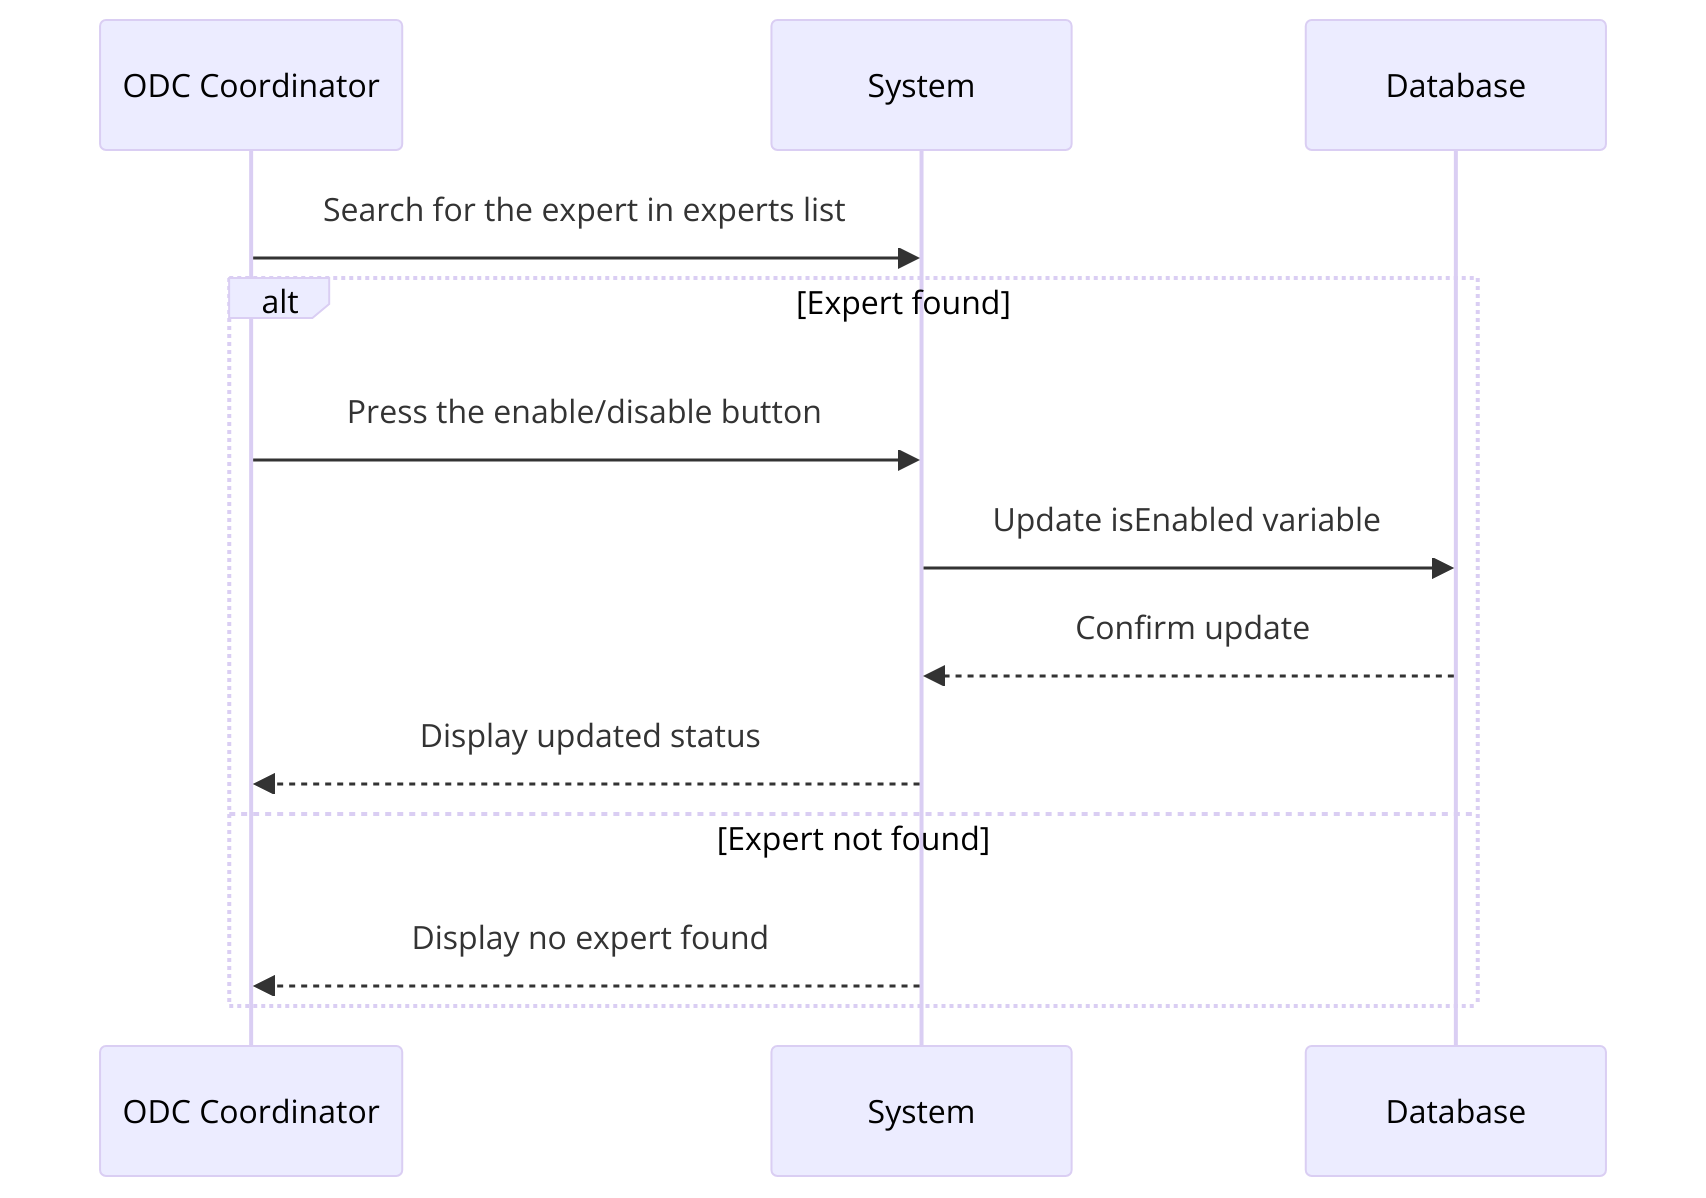
\includegraphics[width=0.8\textwidth]{images/diagram seq3.png}
    \caption{the sequence diagram for the use case 'Enable/Disable ODC Expert'}
    \label{fig:the sequence diagram for the use case 'Enable/Disable ODC Expert'}
\end{figure}



